% Preamble
% ---
\documentclass{article}

% Packages

% \usepackage{graphicx}
% \usepackage{subfig}

\usepackage{multicol}
\usepackage{float}

\usepackage{tikz}
\usepackage{pgfplots}
\usepgfplotslibrary{external}
% \usetikzlibrary{shapes.geometric, arrows}
% 
% \usepackage[english]{babel}

\usepackage{geometry}
\geometry{margin=1.2cm}

% ---

% \graphicspath{ {assets/} }

% \setlength{\columnsep}{1.3cm}

% \setlength{\columnsep}{0.8cm}
\begin{document}
\begin{multicols}{2}

\section{Introduction}

\section{Serial Optimisation}

The first step to improving the was to reduce the number of memory fetched
which took place. In the original implementation 3 parses took place over the
cells dataset which required multiple fetches of the same sections of memory.
To reduce this the 4 parses were fuzed into a single loop. The number of copies
from \verb|cells| to \verb|tmp_cells| was reduced. This was achieved by using
\verb|tmp_cells| as the final answer space for a given timestep (ensuring cells was
never changed) and then swapping \verb|tmp_cells| and cells at the end of the
timestep.

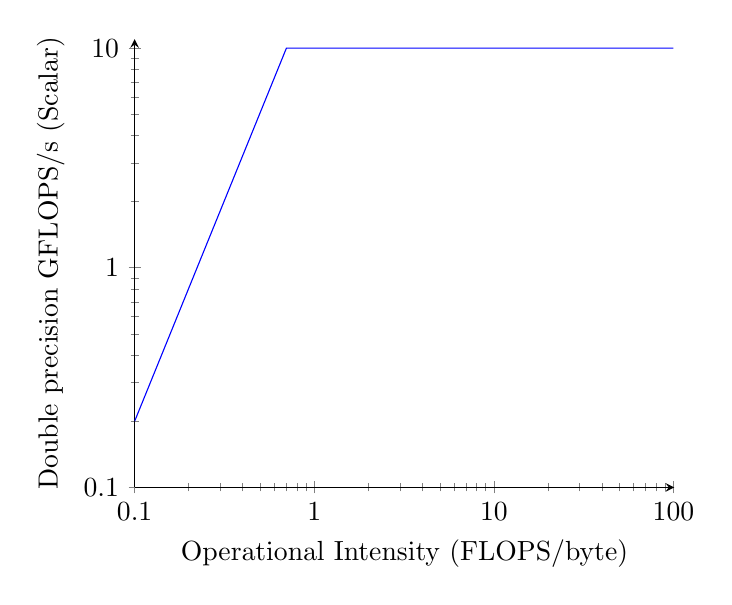
\begin{tikzpicture}
\begin{axis}[
  xmode = log,
  ymode = log,
  axis lines = left,
  xlabel = Operational Intensity (FLOPS/byte),
  ylabel = Double precision GFLOPS/s (Scalar),
  ymin = 0.1,
  xmin = 0.1,
  ymax = 11,
  xmax = 101,
  log ticks with fixed point,
]
\addplot[color=blue] coordinates {
  (0.1, 0.2)
  (0.7, 10)
  (100, 10)
};
\end{axis}
\end{tikzpicture}

\section{Vecotrisation}

The first step to vectorizing the code is to ensure all the array used in
timestep are aligned. This can be achieved by using \verb|__mm_malloc| and then
adding compiler directives which covey this alignment.


\end{multicols}
\end{document}

